\section{Iterative learning control}
Iterative learning control is an effective scheme used to improve repeatedly executing system performance \cite{ILC:2018}. Since torque pulsations were found to be periodic, ILC can be used to learn from previous iterations, thus making it possible to identify torque pulsations automatically. ILC based compensator can be used to reduce the ripple with weak process knowledge \cite{ILC:2007}, which makes the method well suited when numerous systems require compensation.

%"It is human to make mistakes, but it is also human to learn much from experience" \cite{ILC:1984}. This concept was adopted in robotics and further extended to relative fields. The idea is to utilize measurement data to automatically improve the performance of future actions. With robot manipulators, this idea has been used to automatically correct manipulator trajectories \cite{ILC:1984, ILC:1998}. With a PMSM, the reflection process can be used to overcome inevitable disturbances coming from cogging torque, flux harmonics and current measurement errors. The automatic learning can be achieved by implementing an iterative learning controller. The controller can produce satisfying results even with weak process knowledge \cite{ILC:2007}, which makes the scheme well suited for disturbance compensation with various PM machines and systems.

% Antidisturbance ability is weak \cite ILC:2018

% ILC citations:
% Arimoto:       ILC:1984
% Book:          ILC:1998
% P-type         ILC:1990
% Panda 1st      ILC:2004
% Panda 2nd      ILC:2005
% ILC survey     ILC:2007
% Angle-based    ILC:2012
% Airplane grid: ILC:2013
% Robust ILC:    ILC:2018

% ILC special ICL:2000 - delete?


\subsection{ILC prerequisites}

For ILC to be effective, the following postulates must hold \cite{ILC:Book2007, ILC:2012, ILC:1998}
\begin{itemize}
  \item[1)] Every iteration ends in a fixed time duration.
  \item[2)] System invariance is ensured throughout repetition.
  \item[3)] The system output is measured in a deterministic way.
\end{itemize}
In addition to previous postulates, a few system related considerations should be accounted. The measured speed (or torque) must not be filtered too heavily, as this introduces compensation delay. Too great delay can annihilate applied compensation. Since ILC learns from previous iterations, memory storage is required. The memory is accessed frequently, which advocates use of random access memory (RAM). The required memory size depends on compensation accuracy that is being pursued. In addition to free memory space, also processing power is needed for computing compensation values.

%In order to give some insight of the required size, the scale is likely to be hundreds or few thousands of floating point numbers.

%The iterative learning control must fulfill the six axioms listed below \cite{ILC:1998}. Axioms A3-A5 have been relaxed (hence apostrophe). Relaxing the original conditions is necessary for practical systems that incorporate various disturbances \cite{ILC:1998}.
% From the book:
%\begin{itemize}
% \item[A1.] Every trial ends in a fixed time of duration $T > 0$.
% \item[A2.] A desired output $y_d(t)$ is given a priori over that time with duration
%$t \in [0,T]$.
%\item[A3'.] The system is initialized at the beginning of each operation within an error level $\epsilon_1 > 0$, i.e.,
%$$\lVert x_i(0) - x_0\rVert \leq \epsilon_1 \; \text{for} \; i=1,2,...,.$$

%\item[A4'.] The norm of input disturbance $\eta_i(t)$ induced during repeated trials is limited to some extent, i.e., $\lVert\eta_i\rVert \leq \epsilon_2$.
%\item[A5'.] The output $y_i(t)$ can be measured with small noise, i.e., the output error is subject to $$e_i(t) = y_d(t) - \{y_i(t) + \zeta_i(t)\}$$
%where the $L^2$-norm of noise $\zeta_i$ must be small, say $\lVert \zeta_i \rVert \leq \epsilon_3$.

%\item[A6.] The system dynamics are invertible, that is, for a given desired output
%$y_d(t)$ with a piecewise continuous derivative, there is a unique input $u_d(t)$
%that excites the system and yields the output $y_d(t)$.

%Then the problem is to find a recursive control law
%$$u_{i+1}(t) = F(u_i(t), e_i(t))$$
%\end{itemize} 

\subsection{Ripple minimization concept}

The torque pulsations can be negated by generating an opposing torque. This can be done by computing a correction term, which is injected to a control reference. Ideally, the term has the same magnitude but opposite sign as pulsating torque at some time instant. This creates destructive interference which cancels out pulsations.

Disturbances were found to be periodic, which allows them to be identified iteratively. Identification can be done comparing the measured output value with the reference value. In practice, an error can be calculated by subtracting the measured speed from the speed reference and then the task of ILC is to minimize the error by injecting an appropriate correction term. The correction value can be injected either into torque reference \cite{ILC:2004} or to q-axis current reference \cite{ILC:2005, ILC:2018} similarly to Fig. \ref{Compensator_control_diag}. ILC tracks complete periods, which allows it to iteratively find appropriate correction terms for every step.

The minimization concept is easy to understand from examples. A simulation result in Fig. \ref{fig:ilc_concept} shows compensation of arbitrary pulsations. The green signal in plots represents torque produced by the ILC compensator. The blue signal is the pulsating torque, which represents only the sixth harmonic for the sake of clarity. Pulsations are summed to ideal electromagnetic torque, thus leading oscillations of the red signal. Since ILC is disabled in the upper plot, no compensating torque is produced and torque pulsations are directly visible from the actual torque. In the lower plot, ILC is enabled and compensating torque is produced. Now actual torque has smaller amplitude than pulsating torque, which allows to deduce that the compensator reduces torque pulsations. It can be observed that the compensating signal has roughly the same amplitude as actual torque in the upper plot while the phases differ by $\pi$. As a result, majority of torque pulsations cancel out. Part of pulsations remain due to introduction of robustness coefficient \cite{ILC:1990, ILC:2004, ILC:2005}, which will be explained later.
\begin{figure}[htb] 
    \centering
    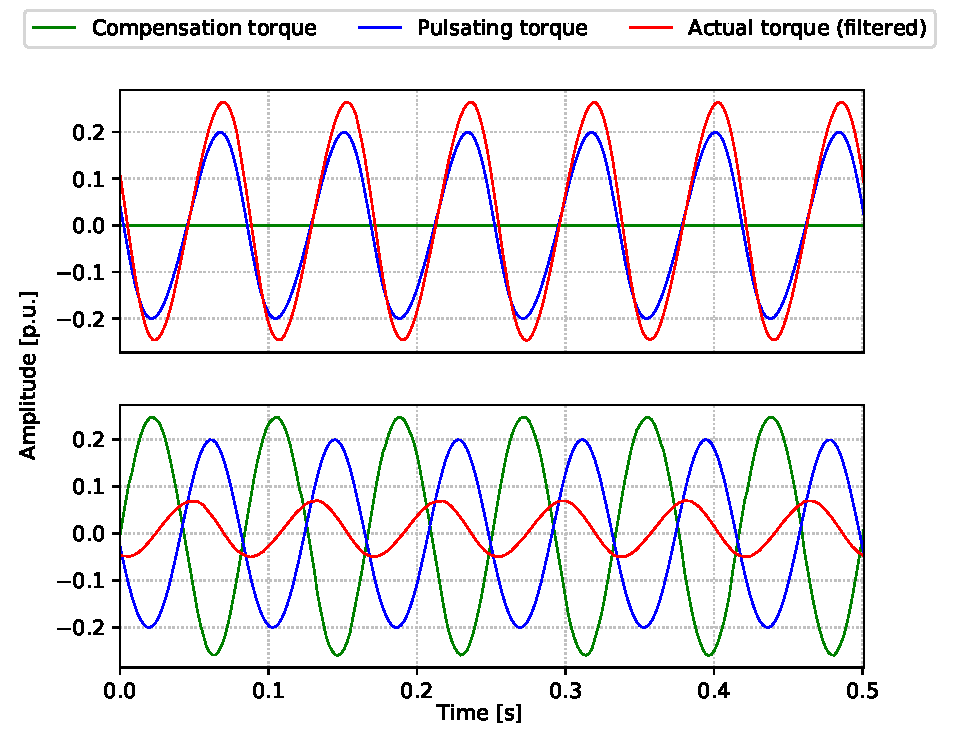
\includegraphics[width=\textwidth]{images/ilc-concept.pdf}
    \caption{The upper figure shows arbitrary torque pulsations, that are reduced in the lower figure, due to simulated destructive interference caused by the ILC compensator}
    \label{fig:ilc_concept}
\end{figure}

Figure \ref{fig:ilc_concept2} illustrates retrieval and improvement process of compensation values. Previous iteration execution is shown with dashed lines, whereas solid lines correspond to current iteration. Compensation torque has been too small on the previous iteration, thus letting the speed to oscillate and induce error between the reference and the measured value. ILC has detected the speed error and it is improving the compensation waveform by increasing amplitude of the compensation pattern. The old compensation values are getting replaced with new values. Due to improved compensation, the speed oscillations have gotten smaller on the current iteration. The ILC compensator is able to retrieve compensation values consistently from the memory by utilizing measured rotor angle. The compensation pattern consists of numerous discrete values that are saved into the memory. It will be discussed how the compensation values can be computed mathematically in the next subsection.
\begin{figure}[htb] 
    \centering
    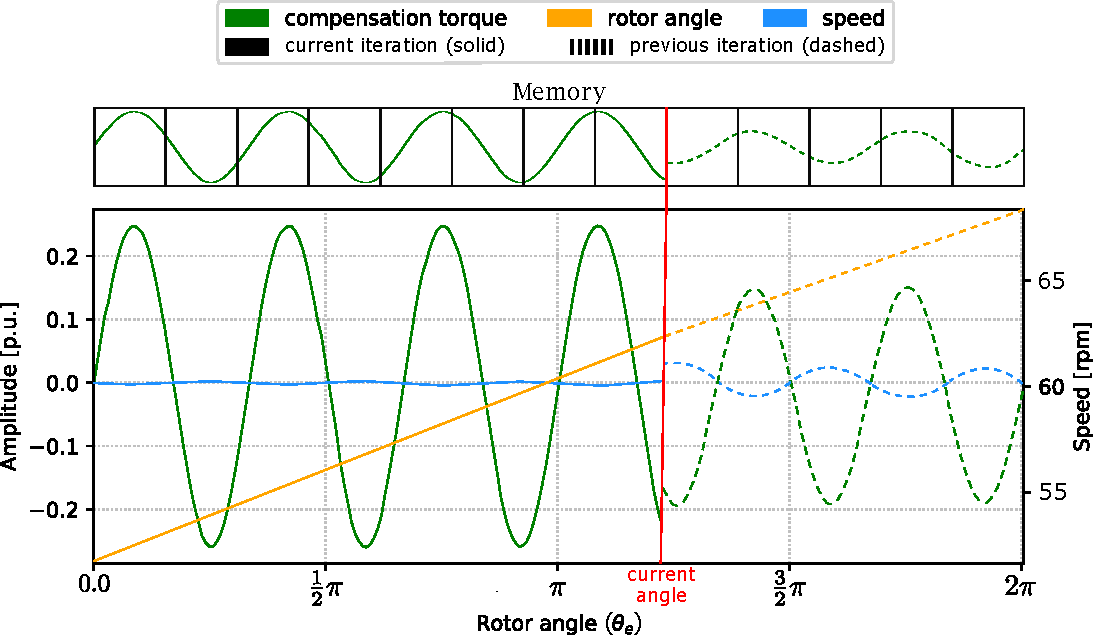
\includegraphics[width=\textwidth]{images/compensation-scheme.pdf}
    \caption{Iterative learning concept of the ILC compensator}
    \label{fig:ilc_concept2}
\end{figure}


\subsection{Iterative learning control algorithm}
ILC is not a single algorithm, but instead, a methodology consisting of many update laws. The vast majority of ILC literature focuses on either proportional type (P-type) or derivative type (D-type) update laws \cite{ILC:1998}. Since unnecessary noise build-up in this problem can be avoided by selecting the P-type update law over the D-type \cite{ILC:2005, ILC:2018}, the focus shall be on a P-type learning controller. In addition, various P-type controllers have been already applied successfully for the speed ripple minimization problem \cite{ILC:2004, ILC:2005, ILC:2012, ILC:2018}.

The learning law is given by \cite{ILC:2005, ILC:2004}
\begin{equation}
    u_{i}(\theta) = (1 - \alpha)u_{i-1}(\theta) + \Phi e_{i-1}(\theta) + \Gamma e_{i}(\theta)
    \label{ILC_update_law2}
\end{equation}
where $\theta$ is the rotor angle, which can be either mechanical or electrical as there is relation between the two. $\Phi$ and $\Gamma$ are gains used to tune controller, $e$ is the speed error and $u$ is control action, which in this case corresponds the current reference correction signal $i^{corr}_{q,i}$. The iteration index $i = 1,2,3,...$ corresponds either mechanical or electrical period depending on whether mechanical or electrical rotor angle is used. The first measurable error is $e_i$ and $e_{i-1}$ can be obtained from memory after one period. Values in the memory can be initialized to zero \cite{ILC:2004}. Figure \ref{fig:ILC_angle_block} visualizes the structure of the ILC algorithm.
\begin{figure}[b]
    \centering
    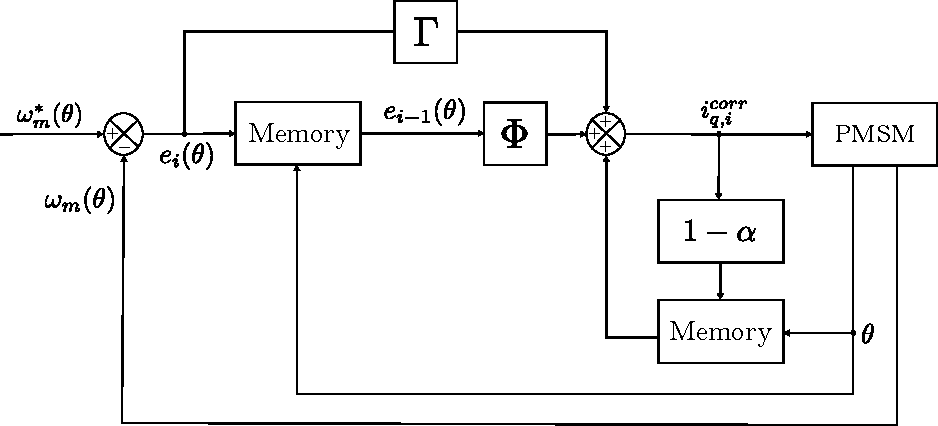
\includegraphics[width=1.0\linewidth]{images/Angle_based_ILC.pdf} 
    \caption{Block diagram of rotor angle-based ILC}
    \label{fig:ILC_angle_block}
\end{figure}

Forgetting factor $\alpha$ can be used to make the P-type algorithm more robust against noise, initialization error and system dynamics fluctuation \cite{ILC:1990, ILC:2005}. Therefore, the parameter $\alpha$ is included into learning law, as this is expected to improve the performance of the controller with real systems. For the same reason, also present error signal $e_{i}(\theta)$ is included, in addition to typical previous iteration error $e_{i-1}(\theta)$, as this should stabilize the learning in presence of perturbations \cite{ILC:2004}.

%and pseudocode is given in Algorithm \ref{Pseudo_ILC}.
%\fontsize{11}{15}
%\begin{algorithm}[htb]
%	\caption{Constant speed ILC}
%	\begin{algorithmic}[1]
%	    \State Initialize, t = 0, \textbf{U} = \{0\}, \textbf{e} = \{0\}
%	    \State $e_{i+1} = \omega_{ref} - \omega_{act}$ 
%		\State $u_{i+1} = (1 - \alpha) \; u_i[t] + \Phi e_i[t] + \Gamma e_{i+1}$
%		\State $\textbf{U}[t] = u_{i+1}$ \algorithmiccomment{Update memories}
%		\State $\textbf{e}[t] = e_{i+1}$
%		\State $t = t < last\_memory\_idx \; ? \; t + 1 : 0$ 
%		\State return $u_{i+1}$
%	\end{algorithmic} 
%	\label{Pseudo_ILC}
%\end{algorithm}

% Obviously it is not possible to know the error in future, thus in practice the update law is delayed with one iteration.

%Visual representation of the algorithm is given in Fig. \ref{Fig:ILC_block}.

%\begin{figure}[htb]
%    \centering
%    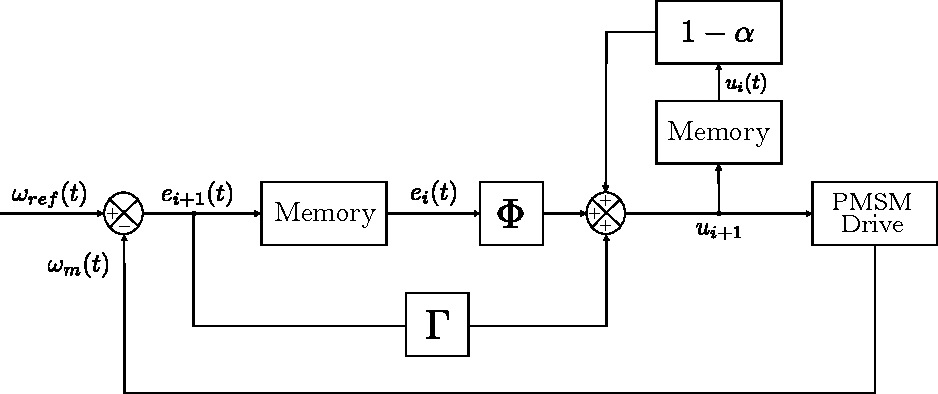
\includegraphics[width=1.0\linewidth]{images/ILC_block_diagram.pdf} 
%    \caption{Block diagram of the P-type ILC with a forgetting factor \cite{ILC:2005}}
%    \label{Fig:ILC_block} 
%\end{figure}


%ILC requires rewritable and fast access memory, such as RAM. This can be reasoned from the update law \eqref{ILC_update_law1} as the previous control action and error are needed for calculating the next action. It is good to note that the previous action refers to the action that was used one period ago, instead of being the most recently computed action. Therefore, the memories must hold values for at least one period. This requirement is easy to fulfill, if the speed stays constant as the required memory size can be calculated by using step size and length of the period. If the speed can change, then satisfying the requirement gets much more difficult. With constant sampling rate, the memory size would need to vary. One period takes more time at slow speed than it takes at high speed. As a result, an enormous amount of memory could be needed at slow speed, which makes time based ILC impractical. Furthermore, not all embedded devices have dynamic memory, so changing the buffer size on the fly might be impossible. Thereupon, ILC update should not be done with respect to time.

%Angle based ILC has relation to the rotor angle instead of time. The angle can be either mechanical or electrical as there is connection between the two. This allows the update law to be rewritten as \cite{ILC:2004, ILC:2012}
%\begin{equation}
%    u_{i+1}(\theta) = (1 - \alpha)u_i(\theta) + \Phi e_i(\theta) + \Gamma e_{i+1}(\theta)
%    \label{ILC_update_law2}
%\end{equation}

%\begin{figure}[htb] 
%    \centering
%    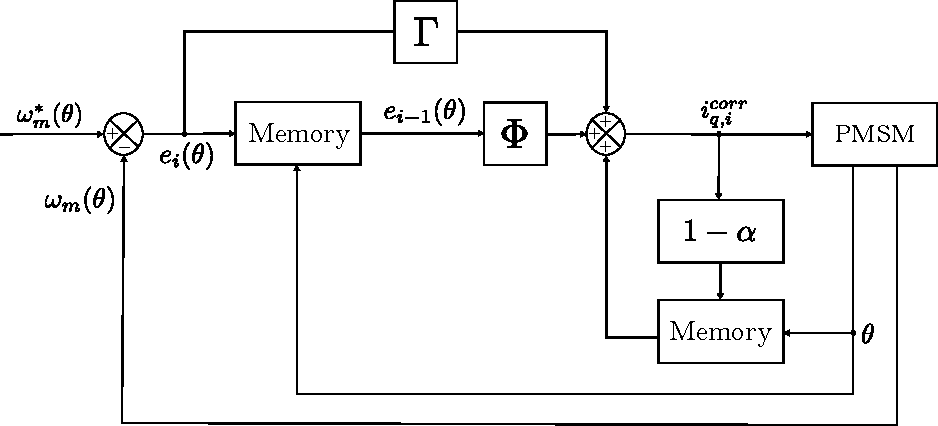
\includegraphics[width=1.0\linewidth]{images/Angle_based_ILC.pdf} 
%    \caption{Block diagram of the constant-speed and the variable-speed ILCs}
%    \label{Fig:ILC_angle_block}
%\end{figure}

The memory usage can be adjusted as long as the memories hold values at least for one full period. Since period length depends on running speed, this leads to the situation where different memory sizes would be needed for different speeds, if memories were accessed with time directly. For this reason, the update law is written with respect to rotor angle, as this allows to have fixed memory size. By quantizing one period into $N$ steps, the values can be stored into memory holding $N$ values. Thus, step size selection has direct effect to memory consumption as well as to compensation performance. The performance suffers if steps are too large, since the algorithm cannot track error accurately.

The fixed size memory is accessed by utilizing rotor angle. Rotor angle quantized to $k$ indices is given by, i.e., $\theta_k = 2\pi k / N$ \cite{ILC:2012}. The measured rotor angle can be associated to an index by using rounding rule, $k = $round$(N \theta / 2 \pi)$ \cite{ILC:2012}. Use of the index $k$ allows reading and writing to desired memory locations. The same element can be consistently retrieved from the memory every period, hence allowing improvement to happen iteratively. It should be noted that quantization makes it possible to leap over values, especially in case of high speed and many steps. The skipped values should be linearly interpolated \cite{ILC:2012}.

The gain values $\Phi$ and $\Gamma$ should be selected carefully to allow converge. Convergence condition for the controller can be derived starting from the torque equation \eqref{torque_eq3} and the final condition is given as \cite{ILC:2004}
\begin{equation}
    \left| \rho \right| = \left| \frac{1-\alpha - k_t \Phi}{1 + k_t \Gamma} \right| < 1
\end{equation}
Since $k_t$ > 0, the condition is satisfied with \cite{ILC:2004}
\begin{equation}
    0 < \alpha + k_t \Phi < 2
\end{equation}
If the torque constant $k_t$ is unknown, its upper bound must be estimated in order to set a value for $\Phi$. Prudent upper bound estimate guarantees convergence for a wider range of $k_t$, but also leads to slower convergence rate \cite{ILC:2004, ILC:2005}. Finding a good value for $\Phi$ is important as it considerably affects the compensation performance. The gain $\Gamma$ influences compensator response between iterations \cite{ILC:2005}. Too large $\Gamma$ will cause oscillatory response, hence, a prudent estimate of $\Gamma \leq \Phi$ may suffice for producing satisfying results \cite{ILC:2004}. However, better compensation performance can be achieved by carefully tuning the controller, instead of using the prudent tuning guidelines.

It can be speculated whether the use of mechanical rotor angle in ILC could provide better compensation results than electrical rotor angle. Mechanical rotor angle allows ILC to observe all possible manufacturing imperfections occurring on one full rotation. Electrical period is only a fraction of mechanical, so asymmetry between poles cannot be fully accounted. However, a shorter period allows to have smaller memory sizes and theoretically ILC should learn faster, because iterations take less time. This gives a good reason to favor electrical angle over the mechanical. During experimental tests, it was observed that use of electrical angle also allows to set slightly higher ILC gains, before instability is encountered. As a direct consequence, the implementation using electrical rotor angle performed slightly better than identical mechanical rotor angle based implementation.

%P-type ILC provides effective steady-state harmonic compensation due to its repetitive action, but does not produce a good transient performance \cite{ILC:2013}. This is why P-type ILC is often combined with conventional PI controller, which handles the transients while ILC is being disabled during the transient.

%{\color{blue} $T_m$ based ILC problem. Often torque transducer is not available, so the torque has to be estimated. Estimated torque is too noisy to be used in compensation. Transducer is expensive investment for a customer...}

%Angle based ILC compensator is described in Fig. \ref{ILC_block}. The ILC compensator can use either electrical or mechanical rotor angle \cite{ILC:2018}. Mechanical angle should provide better compensation results, because ILC perceives imperfections from full mechanical cycle instead of a fraction of it. This is because electrical period is shorter than mechanical, so all manufacturing imperfections cannot be detected when using electrical angle. However, the shorter period is also the strength of electrical angle based compensator. The memory blocks can be smaller because fewer amount of numbers needs to be stored in them. Additionally, the convergence happens faster with shorter iterations and therefore the compensator using electrical angle should dampen the ripple faster. favoured over mechanical angle.

%{\color{blue}TODO: check does my ILC use electrical or mechanical angle for memory update. Uses electrical: fix diagram...}

% These methods improve compensation, but may introduce other undesired effects
% Chattering effect - sliding mode observer

%\subsection{Practical limitations}
%{\color{blue} How about writing practical limitations? This is relevant.}

%\begin{itemize}
%  \item Gain tuning can be challenging
%  \item Buffer size has a direct effect to performance
%  \item Either actively learns or then doesn't learn at all
%  \item What if the produced torque needs to be periodic?
%  \item High speed performance is not good...
%  \item chattering?
%  \item doesn't work if noisy signals = doesn't work with bad resolvers.
%  \item Cannot be used in transienst (gain table - gains must be actively changed)
%  \item Gain scheduling (testing takes effort. Cannot be calculated easily)
%\end{itemize}


%Sliding-mode observer was used in \cite{ILC:2018} and \cite{ILC:2004}, yet it introduced chattering. Although the studies were able to overcome the chattering problem, introducing new nuisances does not seem correct direction. Therefore, it will be concluded that observer based compensation may work, though there are likely to be better approaches.

% Encoder measurement noise:
% The array size can change every iteration due to noise and then memory exceeds

% It can be speculated whether the mechanical angle could provide better compensation results than the electrical angle, since the ILC should be able to observe all possible manufacturing errors occurring on one full rotation. Electrical period is only a fraction of mechanical, so asymmetry between poles cannot be fully accounted. However, a shorter period allows to have smaller memory sizes and theoretically the ILC should learn faster, because iterations take less time. This gives a good reason to favor electrical angle over the mechanical. During experimental tests, it was additionally observed that electrical angle based ILC has better compensation performance than identical mechanical angle based ILC. It appears that surprisingly the generalization coming from electrical periods may have positive effect when the signals are noisy.



%which is beneficial. Moreover, it was experimentally 
%since mechanical period equals one whole rotation. Electrical period is only a fraction of mechanical, so symmetry is being assumed. Intrestingly, it was found that electrical ...better results ... and takes less memory space as ... period is shorter.

% The ILC implementation had two array with 750 elements and each element having 32 bit accuracy. It can be calculated that 48 kB are needed to store the arrays. 

\clearpage
